%%% This LaTeX source document can be used as the basis for your technical
%%% report. Intentionally stripped and simplified
%%% and commands should be adjusted for your particular paper - title, 
%%% author, citations, equations, etc.
% % Citations/references are in report.bib 

\documentclass[conference]{acmsiggraph}

\usepackage{graphicx}
\graphicspath{{./images/}}
\newcommand{\figuremacroW}[4]{
	\begin{figure}[h] %[htbp]
		\centering
		\includegraphics[width=#4\columnwidth]{#1}
		\caption[#2]{\textbf{#2} - #3}
		\label{fig:#1}
	\end{figure}
}

\newcommand{\figuremacroF}[4]{
	\begin{figure*}[h] % [htbp]
		\centering
		\includegraphics[width=#4\textwidth]{#1}
		\caption[#2]{\textbf{#2} - #3}
		\label{fig:#1}
	\end{figure*}
}


\usepackage{lipsum}

\TOGonlineid{45678}
\TOGvolume{0}
\TOGnumber{0}
\TOGarticleDOI{1111111.2222222}
\TOGprojectURL{}
\TOGvideoURL{}
\TOGdataURL{}
\TOGcodeURL{}

\title{Performance Analysis of Real Time Multi-platform Physics Simulations \\
	   Final Report}

\author{Sam Serrels\\\ 40082367@napier.ac.uk \\
Edinburgh Napier University\\
Physics-Based Animation (SET09119)}
\pdfauthor{Sam Serrels}

\keywords{Multi-platform Physics, Optimisation, GPU, Cell, PS3}

\begin{document}

\teaser{
   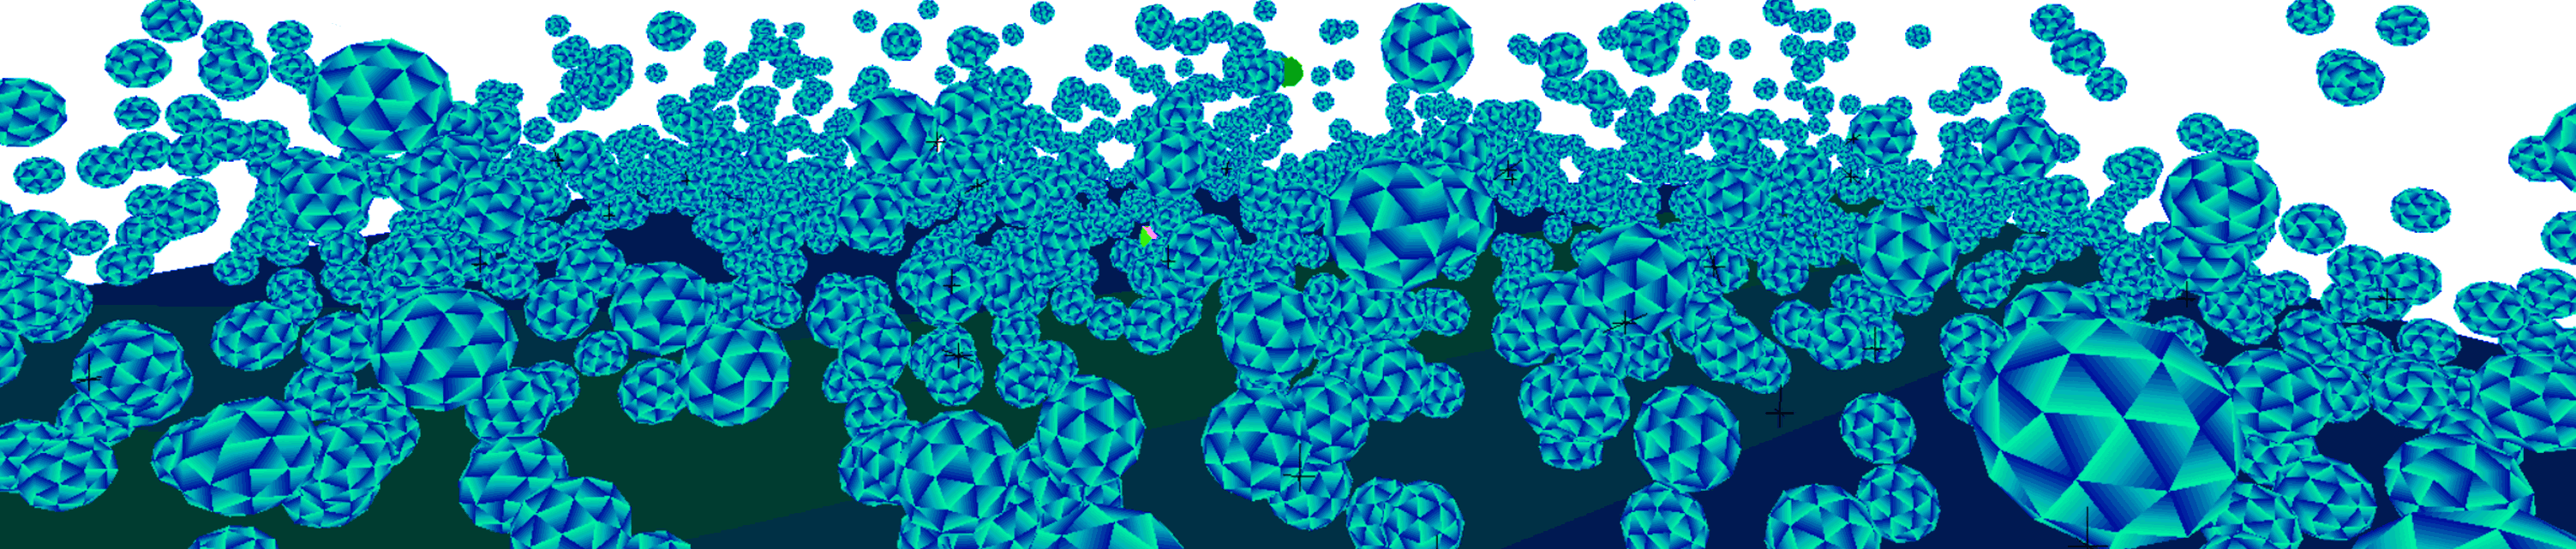
\includegraphics[height=1.5in]{images/sampleteaser}
   \caption{Project screenshot}   
 }		

\maketitle

\begin{abstract}
This project aimed to develop a physics engine and simulate a scene consisting of thousands of bouncing balls, running on various systems, such as the Sony Playstion 3.
The performance of each system was measured as the systems were optimised and are compared in this final report.
\end{abstract}

\keywordlist
%\copyrightspace

\section{Introduction}

\paragraph{Project Aims}
This project attempted to create a physics solution that would run on various systems, along with a game engine with an appropriate interface to swap in other existing physics solutions. 
The target platforms were the Sony Playstation 3, and a conventional x86 multi-core PC architecture.

\paragraph{Simulation}
The scene that is simulated is a large set of Bouncing balls, a scenario picked for it's large potential for parallelisation and general visual appeal. The inspiration for this came from a television advert where thousands of bouncing balls were thrown down a sloped street.

\section{Background / Related Work}
Real-time physics on a Playstation 3 is exclusively used in video games, where speed and resource optimisations take priority over simulation accuracy. Often the physics solutions are tailor made for each visual effect, full general physics solvers are rare. Only games which rely on physics as a gameplay element devote much processor time to physics.
PC exclusive titles tend to take a more relaxed approach to physics, due to the extra resources available. Games may use a full physics sovler just for aesthetic value with no additional gameplay mechanics. This can also be a causation of a multitude of physics libraries available for the PC platform.

\figuremacroW
{balls2}
{Project Inspiration}
{\protect\cite{advert}}
{0.96}

\section{Software Design}
Methodology/Software design/logic control. You are expected to do some software
modelling of your physics-based animation choice. At a minimum you are expected to
provide some state modelling and sequence modelling. Avoid providing simple models just
to fill in this section, and only highlight some of the core functionality.

\subsection{Project Design}
The solution is split into three projects: Physics, Engine, and Game.
\paragraph{Game}
The Game project is the highest level, it has no need to understand how the Engine works, or what platform the code is running on. This is where the simulation scene is created, with all the balls initialised. This project also hosts the Main function, the program entry point; where the main game loop is created an run.

\paragraph{Engine}
The code within the Engine project is responsible for managing all the internal systems and platform specific code. The structure is designed to maximize code reuse across the platform code, while minimizing the need for including preprocessor checks. Interface classes are used extensively to abstract the platform code as much as possible from each subsystem, this does result in a large amount of extra classes, but the benefit of code clarity in each class outweighs the negative cost of more files for this size of project.

\paragraph{Physics}
This is where all the physics code is written and executed. The Library supports Plane, Sphere and cuboid shapes for rigid body simulation. These shape objects are created by the Engine and synced with the enties object used for rendering every frame. The physics library keeps track of every object created in a collection called a scene.

The Engine and Physics Projects are compiled as a library, and linked with the Game project.

\paragraph{Engine Entity component Model}
The Engine stores render objects as Entities, each of which has a set of components attached to it.
The components used in this project are a Mesh renderer component, a camera component, a keyboard movement component and the three set of physics shapes as components. The base entity class only stores  position, rotation and housekeeping data.
This follows the entity component model, which allows for complex combinations of entities, without the need for complex inheritance trees.

\paragraph{Engine Modularity}
Each system of the engine has been designed with as little dependency on each other as possible. This is enforced strongly for the low level rendering classes, as these have the least amount of shared code across platforms. The interface between the Engine and the Physics project is set-up so another physics library could be used with only a small wrapper class needed for each new library.

\figuremacroW
{physicsclasses}
{Physics Dependency Graph}
{Forward decelerations are used to minimize header co-dependency throughout the project}
{1.0}

\subsection{Physics}
\paragraph{Design of Physics Library}
The Physics library is rather small compared to the Engine library, it makes use of the same maths library and utility classes, allowing for easy transfer of data between the systems. The physics system has a single "Scene" which hosts all the "Physics Objects" which take the form of the different rigid body shapes.

\paragraph{Physics Process}
There are multiple physics updates or "Ticks" every frame. The time the simulation uses as the the time between ticks is constant, in this project the tickrate	is set to a 100th of a second. The amount of ticks per frame depends on how much real time has passed between frames and the tickrate.\\	
At the start of each tick, the first process is collision detection. This checks every object against evy other object. Spacial partitioning is used to narrow this search space down to only check for collisions against objects that are near each other.
\\
Collision Detection uses the attributes of each physics object to determine if a collision has taken place. If it has, a collision object is created, consisting of information such as the collision normal, penetration depth and position.
\\
Once the detection process is finished, the collision resolver iterates through all of the collisions and calculates an impulse force to apply to each object to push them away from each other.
\\
Finally, each physics object is then "integrated", a process of applying the added forces and rotational torques to the position, velocity and acceleration of each object. Other calculations, such as updating the inertia tensor matrix are also calculated here.

\paragraph{Spacial Partitioning}
To reduce the search set when detecting collisions, spacial partitioning is used. This divides the world into a grid of equally sized virtual containers, this project only uses two dimensions, so the vertical Y dimension is ignored. Each object is placed in a container depending on its position in the world, only other objects within the same container are checked for collision. After all the objects have been integrated, the gird is scanned through and if an objects position has moved out from one container, the grid is updated to reflect this.
\\
The Grid is implemented as a 2D array of Vector pointers, each vector contains pointers to physics object so the memory size used is minimal. The process of determining which container an object is in is based only on it's position, so a simple divide and round maths operation can be used. Therefore the overhead in updating and managing the grid is minimal, and the performance benefits of using it are substantial.
	
\section{Results}
Experimental Results/description of your physics-based simulation implementation
including screen-shots.


\paragraph{Spacial Partitioning Results}
The use of spacial partitioning dramatically increased the performance of the overall simulation, the results can be seen in Figure: \ref{fig:chart1-a} and Figure: \ref{fig:chart1-b}. 
This was an initial implementation, and could be optimised further by varying the size of the sectors and having the grid divide in all 3 Dimensions.

\paragraph{Simulation results}
Profiling the application revealed that the bottlenecks in the simulation reside mostly in the collision detection phase. In the event that there are thousands of simultaneous collisions, the collision resolver code may overtake the detection code in terms of processor time. This can happen at the start of the program, ass the balls start close to each other.

\paragraph{Rendering bottlenecks}
Without physics, on the hardware used to test this project, the maximum number of static spheres that could be rendered was around 20'000. The spheres are loaded in from a model file, each has 240 polygons.

\paragraph{Physics stall}
As the aim of this project was to develop a realtime physics application, with the purpose of integration into a larger game kept in mind, some methods were used to keep the framerate above 60fps. If the total time taken to process the needed amount of physics ticks execde a the total time between frames, the ticks stop being processed and the engine goes straight to rendering. This means that as the framerate lowers due to phsyics computation time, at some point the simulations starts to slow down, as less ticks are processed. This happens around the 100fps mark, the worst case scenario is that a single physics tick would take up more time than the engine can give to physics, in which case the framerate will quickly sink towards 0. This can be observed when the simualtion size exeeds 8000 on Figure: \ref{fig:chart1-b}.


\figuremacroW
{screenshot3}
{Starting position of Simulation}
{Screenshot}
{1.0}

\figuremacroW
{screenshot4}
{Balls after the 3 secons of simulations}
{Screenshot}
{1.0}

\figuremacroW
{screenshot5}
{Close up of Balls}
{Screenshot}
{1.0}


\figuremacroF
{chart1-a}
{Frames Per Second / Amount of Balls}
{Upto 400 balls, spacial partitioning gives no noticeable improvement}
{1.0}

\figuremacroF
{chart1-b}
{Frames Per Second / Amount of Balls (1000+)}
{After 8000, both methods become unplayable with constant physics stalls.}
{1.0}

\section{Evaluation}

\paragraph{Scope}
The results of the project have been inconclusive in determining the performance benefits of physics optimisation accross multiple platforms. The main shortcomming has been the Playstation 3 portion of the project. Due to unforseen technical problems and the time constraints of the project, the support for the Playstion 3 could not be completed to a level which would result in useable results.



Evaluation - An evaluation of your implementation. Points to consider discussing in this
section are:
 A comparison against the original concept
 Comparison against other simulations in the genre, particularly the ones that
inspired your choice
 A discussion on the quality of the simulation
 Possible improvements to your simulation

\section{Future Work}



\bibliographystyle{acmsiggraph}
\bibliography{report}


\figuremacroF
{engineclasses}
{Engine Dependency Graph}
{PS3 Classes are ommitted}
{1.0}

\end{document}